\section{Lecture 6: VLIW Processors}
Good things about SSA:
\begin{itemize}
\item The difference from Superscalar is that in that architecture the hardware solves everything for us.
\item It detects potential parallelism between instructions.
\item It tries to issue as many instructions as possible in parallel.
\item It uses register renaming to increase parallelism.
\item if improvements are made on the design we don't need to change the programs.
\item Old programs can benefit from the additional machine parallelism, since the new hardware will simply issue instructions in a more efficient way.
\end{itemize}

Problems with SSA:
\begin{itemize}
\item The down side though is that the architecture is very complex.
\item A lot of hardware is needed for run-time detection of parallelism.
\item It consumes a lot of power.
\item There is, therefore a limit in how far we can go with this technique.
\item The instruction window for execution is limited in size, this limits the capacity to detect large number of parallel instructions.
\end{itemize}

\subsection{Very Long Instruction Word Processors}
In VLIW architecture, Several operations that can be executed in parallel are placed in a single instruction word as can be seen in figure \ref{fig:vliw-instr}.

\begin{figure}[H]
  \centering
  \scalebox{0.6}{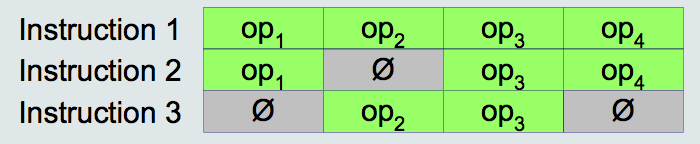
\includegraphics{img/vliw-instr.png}}
  \caption{VLIW instruction word}
  \label{fig:vliw-instr}
\end{figure}

VLIW rely on compile-time detecton of parallelism. The compiler analyzes the program and detects operations to be executed in parallel.
  
After one instruction has been fetched, all the corresponding operations are issued in paralell. The instruction window limitation disappears: the compiler can potentially analyze the whole program to detect parallel operations.

\begin{figure}[H]
  \centering
  \scalebox{0.6}{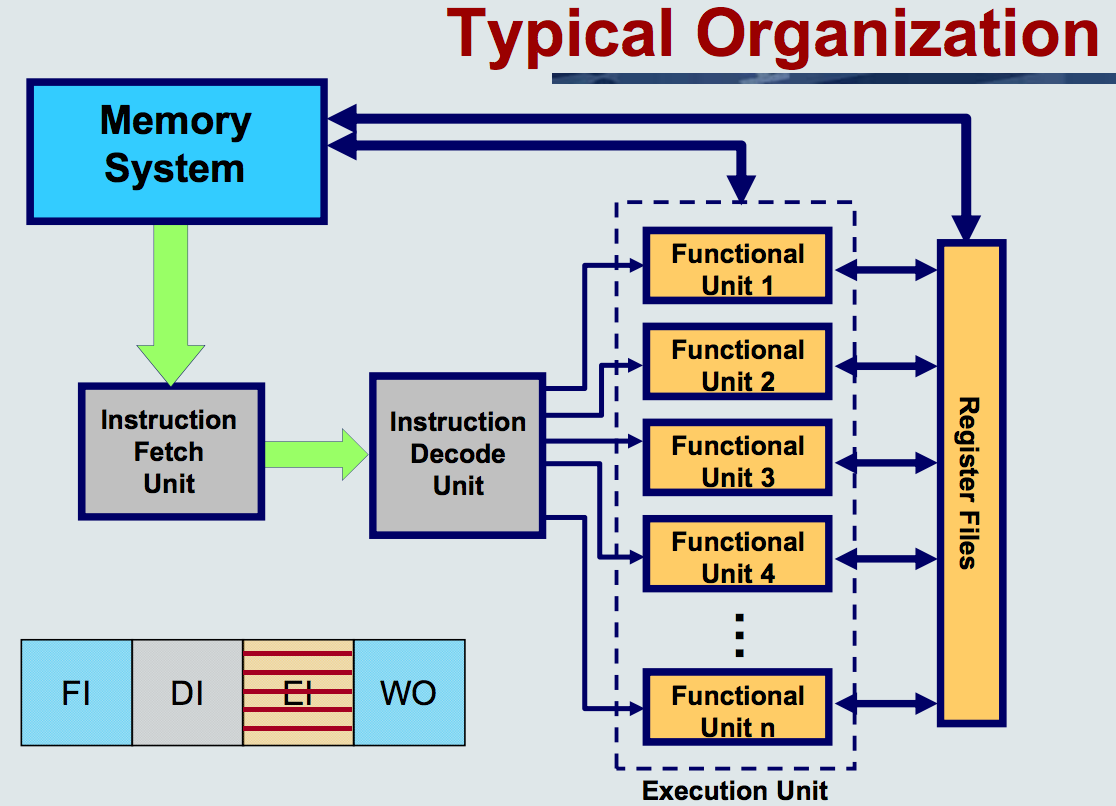
\includegraphics{img/vliw-org.png}}
  \caption{Typical VLIW organization}
  \label{fig:vliw-org}
\end{figure}

\subsubsection{Explicit Parallelism}
Instruction parallelism scheduled at compile time. It is included within the machine instructions explicitly. This means that the hardware is very much simplified, and that functional units can be added withouth need of additional sophisticated hardware to detect parallelism, as in SSA.

An EPIC (Explicitly Parallel Instruction Computing) processor uses this information to perform parallel execution.

As it is the Compiler that determines the parallel operations, this is done off-line and has much more time and is therefore not as time critical as SSA, as this is done at run-time by the hardware in that case. Good compilers can detect parallelism based on global analysis of the whole program.

\subsubsection{Main issues}
But there is also some problems with VLIW aswell.
\begin{itemize}
\item Needs a large number of registers.
\item Large data transport capacity is needed between Fus and the register files and between register files and memory.
\item High bandwidth between instruction cache and fetch unit is also needed due to long iunstructions.
\item Every code block is not optional for the design, which leads to that some FUs might be unused a lot of the time.
\end{itemize}
  
\subsubsection{Software issues}
If a new version of the processor introduces additional FUs, the number of operations to execute in parallel is increased. Therefore, the instruction word changes, and old binary
code cannot be run on the new processor

We might not have sufficient parallelism in the program to utilize the large degree of machine parallelism.
\begin{itemize}
\item Hardware resources will be wasted in this case.
\item  A lot of memory space will also be wasted.
\item A technique to address this problem is loop unrolling, which can be performed by a compiler. 
\end{itemize}

\subsection{Loop unrolling}
\textbf{Loop unrolling}: a technique used in compilers in order to increase the potential of parallelism in a program. It supports more efficient code generation for processors with instruction level parallelism.

What this means is that we will try to re-write loops to eliminate instructions that controls the loop.

An example is given in figure \ref{fig:loop-unrolling}.
\begin{figure}[H]
  \centering
  \scalebox{0.6}{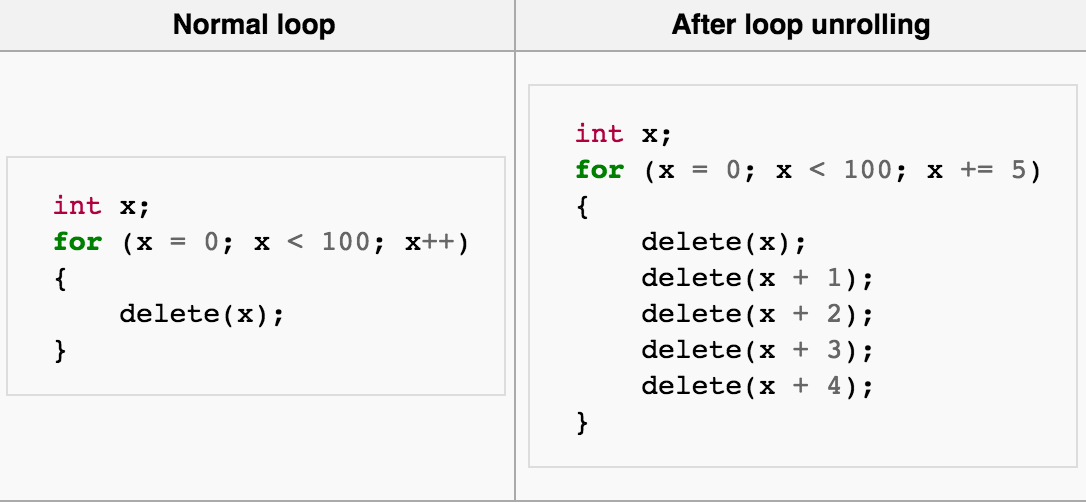
\includegraphics{img/loop-unrolling.png}}
  \caption{A simple example of loop unrolling.}
  \label{fig:loop-unrolling}
\end{figure}

Before using loop unrolling, we have 100 iterations, after we only need 20 iterations. This means that only 20\% of the jumps and conditional branches that were taken before is taken now. What this really does, is that it makes it possible for us to pack the instructions tighter and execute the loop in far less cycles.

But there is also a limit in have many iterations we can unroll, depending on the architecture.

Loop unrolling also increases the amount of:
\begin{itemize}
\item Memory space needed to store the instructions.
\item The amount of register needed to store data for operations that are performed in parallel.
\end{itemize}

\subsection{IA-64 architecture}
The key features of IA-64 are:
\begin{itemize}
\item \textbf{Large number of registers}: The IA-64 instruction format assumes the use of 256 registers.
\item \textbf{Multiple execution units}.
\newline
\end{itemize}

Four types of execution unit are defined in the IA-64 architecture:
\begin{itemize}
\item \textbf{I-unit}:Forintegerarithmetic,shift-and-add,logical,compare,andintegermul- timedia instructions
\item \textbf{M-unit}: Load and store between register and memory plus some integer ALU operations
\item \textbf{B-unit}: Branch instructions
\item \textbf{F-unit:} Floating-point instructions
\end{itemize}

The basic idea of the architecture can be seen in figure \ref{fig:ia64-architecture}
\begin{figure}[H]
  \centering
  \scalebox{0.6}{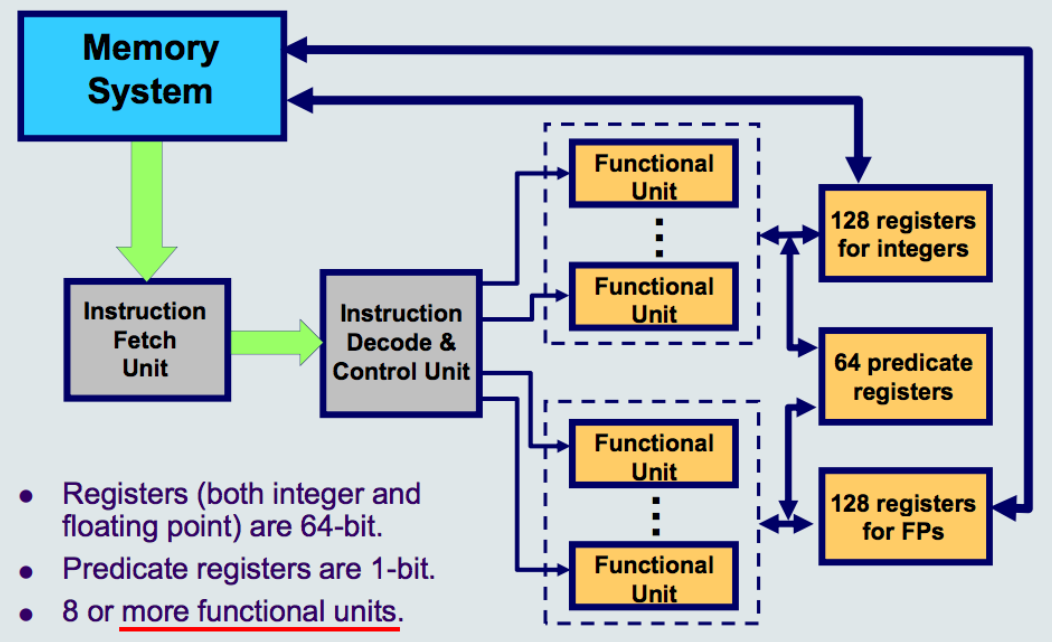
\includegraphics{img/ia64-architecture.png}}
  \caption{IA-64 Architecture}
  \label{fig:ia64-instr-architecture}
\end{figure}


\subsubsection{Instruction format}
In figure \ref{fig:ia64-instr-format} we can see how the instruction format are built.

\begin{figure}[H]
  \centering
  \scalebox{0.6}{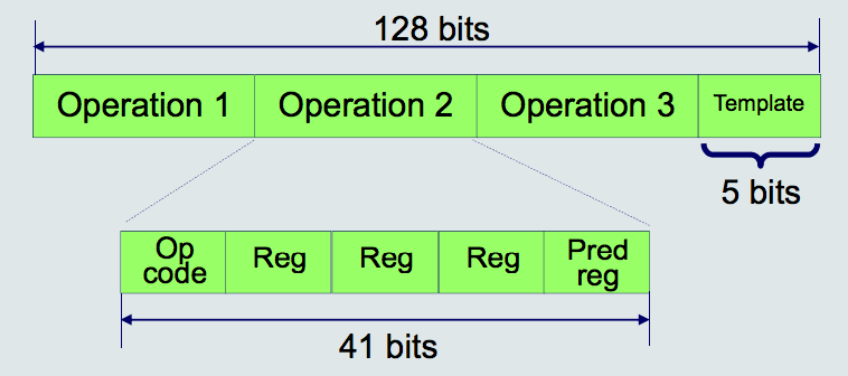
\includegraphics{img/ia64-instr-format.png}}
  \caption{Instruction format forIA-64.}
  \label{fig:ia64-instr-format}
\end{figure}

Three operations are specified in an instruction word, but it's not sure that we can execute them in parallel! This is what we use the template for.

The template tells what instructions in the instruction word that can be executed in parallel, it also connects \textbf{neighboring instructions}. Therefore,
operations from different instructions can also be executed in parallel

The positive things 

\subsubsection{Predicated execution}
\begin{itemize}
\item Any operation can refer to a predicate register. $<$Pi$>$ operation where i is the number of a predicate register (between 0 and 63)
\item This means that an operation is to be committed (the results made permanent) only when the respective predicate is true (i.e., the predicate register gets value 1).
\item If the predicate value is known when the operation is issued, the operation is executed only if this value is true.
\item If the predicate is not known at that moment, the operation will also be started. If the predicate turns out to be false, the operation is discarded.
\item If no predicate register is mentioned, the operation is executed and committed unconditionally
\end{itemize}


\subsubsection{Branch Predication}
We can first note that this is \textbf{not} the same as \textbf{Branch Prediction}.

It is an compiler technique that lets both branches of a conditional branch to be executed in parallel, to increase the amount of parallel instructions.

This is kind of like guessing both answer answers in a yes/no questions. The branch that was correct will then commmit its result and we will just ignore/undo the results of the branch that was incorrect.

This technique of course need duplicated hardware (given by the IA-64 architecture), and it will mean that some of the hardware will be wasted instead of doing something useful.

The upside is that we won't loose any time with branch misses.
\subsubsection{Placement of Loading}
An operation that loads from memory should be placed, so that memory latency is avoided. An example of this can be seen in figure \ref{fig:placement-of-loading}
\begin{figure}[H]
  \centering
  \scalebox{0.6}{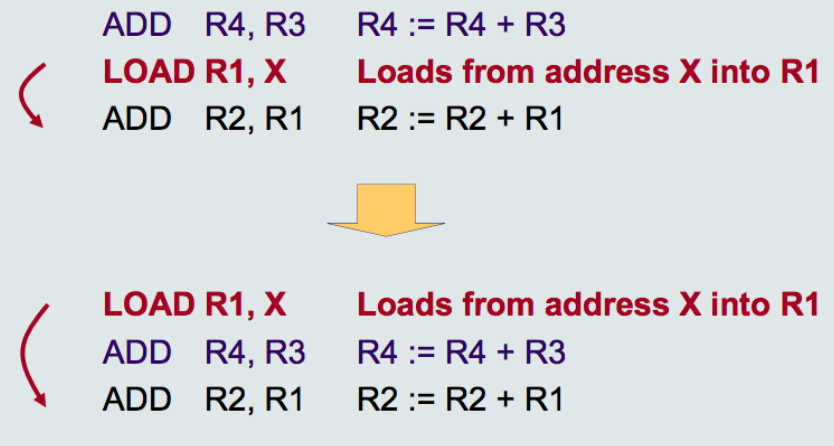
\includegraphics{img/placement-of-loading.png}}
  \caption{We can avoid memory latency by loading from the memory in good time before we need the memory.}
  \label{fig:placement-of-loading}
\end{figure}
\subsubsection{Speculative Loading}
Speculative loading tries to reduce latencies generated by load instructions. It allows load instructions to be moved across branch boundaries (\ref{fig:speculative-loading}), and so page exceptions will be handled only if really needed.
\begin{figure}[H]
  \centering
  \scalebox{0.6}{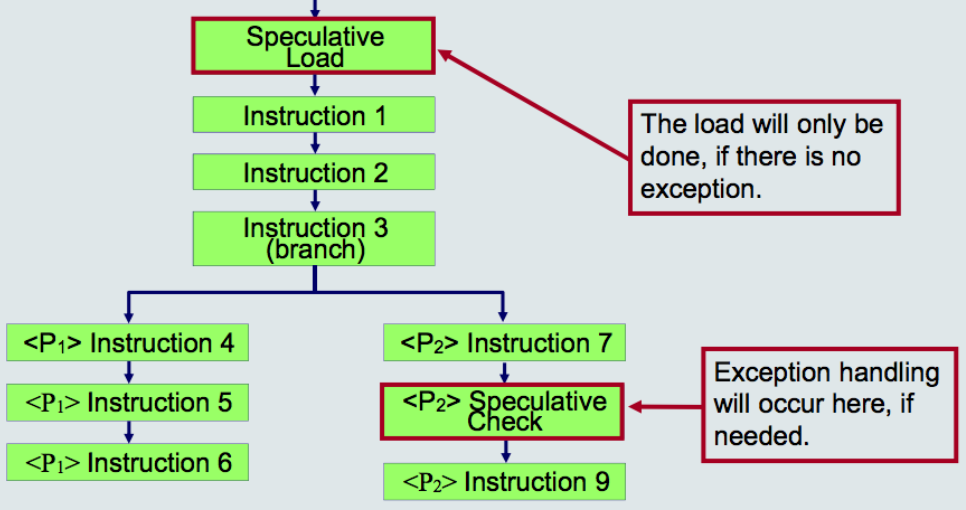
\includegraphics{img/speculative-loading.png}}
  \caption{Speculative loading.}
  \label{fig:speculative-loading}
\end{figure}


